\documentclass{beamer}
%\usetheme{default}
%\usetheme{AnnArbor}
%\usetheme{Antibes}
%\usetheme{Bergen}
%\usetheme{Berkeley}
%\usetheme{Berlin}
%\usetheme{Boadilla}
%\usetheme{CambridgeUS}
%\usetheme{Copenhagen}
%\usetheme{Darmstadt}
%\usetheme{Dresden}
%\usetheme{Frankfurt}
%\usetheme{Goettingen}
%\usetheme{Hannover}
%\usetheme{Ilmenau}
%\usetheme{JuanLesPins}
%\usetheme{Luebeck}
%\usetheme{Madrid}
%\usetheme{Malmoe}
%\usetheme{Marburg}
%\usetheme{Montpellier}
%\usetheme{PaloAlto}
%\usetheme{Pittsburgh}
%\usetheme{Rochester}
%\usetheme{Singapore}
%\usetheme{Szeged}
\usetheme{Warsaw}

\usepackage{graphicx}
\usepackage{booktabs}
\usepackage{xeCJK}
\usepackage{setspace}
\usepackage{listings}
\setCJKmainfont{微软雅黑}
\setmonofont{Monaco}
\begin{document}
\begin{spacing}{1.5}
	\title[现代优化算法]{现代优化算法}
	\author{李琛}
	\institute[FDU]
	{
		Fudan Univerisity \\ 
		\medskip
		\textit{lic.tiny@gmail.com} 
	}
	\date{\today} 

	\begin{frame}
		\titlepage 
	\end{frame}

	\begin{frame}
		\frametitle{Overview} 
		\tableofcontents
	\end{frame}
	
	\section{爬山法}	
	\begin{frame}\footnotesize
		\frametitle{爬山法}
			爬山算法是一种简单的贪心搜索算法,该算法每次从当前解的临近解空间中选择一个最优解作为当前解,直到达到一个局部最优解。\\

         \begin{itemize}
         	\item	局部最优
         	\item	高地:无法确定搜索最佳方向,会产生随机走动,使得搜索效率降低
         	\item	山脊:搜索可能会在山脊的两面来回震荡,前进步伐很小。
         \end{itemize}
		\begin{figure}
			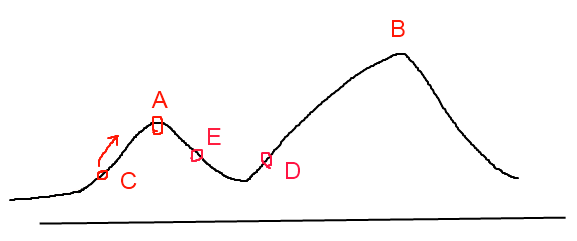
\includegraphics[width=0.7\linewidth]{pic1.png}
		\end{figure}
	\end{frame}
	\begin{frame}
		\frametitle{伪代码}
		\lstset{numbers=left, basicstyle=\scriptsize\ttfamily,
		numberstyle=\tiny, keywordstyle=\color{blue!70}, commentstyle=\color{red!50!green!50!blue!50}, frame=shadowbox, rulesepcolor=\color{red!20!green!20!blue!20},escapeinside=``, xleftmargin=1em,xrightmargin=0.5em, aboveskip=1em}

		\lstinputlisting{climbing.txt}
	\end{frame}
	

	\section{模拟退火算法}
	\begin{frame}\footnotesize
		\frametitle{模拟退火算法}
		模拟退火算法(Simulated Annealing,SA)来源于固体退火原理,将固体加温至充分高,再让其徐徐冷却,加温时,固体内部粒子随温升变为无序状,内能增大,而徐徐冷却时粒子渐趋有序,在每个温度都达到平衡态,最后在常温时达到基态,内能减为最小。 \\
模拟退火算法是基于Monte-Carlo迭代求解策略的一种随机寻优算法,其出发点是基于物理中固体物质的退火过程与一般组合优化问题之间的相似性。模拟退火算法从某一较高初温出发,伴随温度参数的不断下降,结合概率突跳特性在解空间中随机寻找目标函数的全局最优解,即在局部最优解能概率性地跳出并最终趋于全局最优。
	\end{frame}
	\begin{frame}\footnotesize
		\frametitle{算法简介}
			假设材料在状态i下的能量为$E(i)$,那么材料在温度$T$时从状态$i$进入状态$j$遵循如下规律:
			\begin{itemize}
				\item	如果$E(j) \leq E(i)$,接受该转换
				\item	如果$E(j) > E(i)$,则以$e^{\frac{E(i) - E(j)}{kT}}$的概率接受\\其中$K$为玻尔兹曼常数,$T$为当前温度
			\end{itemize}
	\end{frame}
	\begin{frame}\footnotesize
		\frametitle{证明}
			在某一特定温度$T$下,经过充分转换,材料达到热平衡,此时材料处于状态$i$的概率满足玻尔兹曼分布
			$$P_{T}(x = i) = \frac{e^{-\frac{E(i)}{KT}}}{\sum\limits_{j \in S} e^{-\frac{E(i)}{KT}}}$$
			显然
			$$\lim_{T\to\infty}{T}\frac{e^{-\frac{E(i)}{KT}}}{\sum\limits_{j \in S} e^{-\frac{E(j)}{KT}}} = \frac{1}{|S|}$$
			其中$|S|$表示集合$S$中的状态数量
	\end{frame}
	\begin{frame}\footnotesize
		\frametitle{证明}
			温度下降时
			$$\lim_{T\to 0}{T}\frac{e^{-\frac{E(i) - E_{min}}{KT}}}{\sum\limits_{j \in S} e^{-\frac{E(j) - E_{min}}{KT}}} = \lim_{T\to 0}{T}\frac{e^{-\frac{E(i) - E_{min}}{KT}}}{\sum\limits_{j \in S_{min}} e^{-\frac{E(j) - E_{min}}{KT}} + \sum\limits_{j \not\in S_{min}} e^{-\frac{E(j) - E_{min}}{KT}}}$$
			$$ = \lim_{T\to 0}{T}\frac{e^{-\frac{E(i) - E_{min}}{KT}}}{\sum\limits_{j \in S_{min}} e^{-\frac{E(j) - E_{min}}{KT}}} = 
			\left\{
				\begin{aligned}
				&\frac{1}{|S_{min}|}\quad \text{若}i \in S_{min}\\
				&0	\qquad \text{otherwise}
				\end{aligned}
			\right.$$
			

			上式表明,当温度很低时,材料会有很大概率进入最小状态
	\end{frame}
	\begin{frame}
		\frametitle{伪代码}
		\lstset{language=Python,numbers=left, basicstyle=\tiny\ttfamily,
		numberstyle=\tiny, keywordstyle=\color{blue!70}, commentstyle=\color{red!50!green!50!blue!50}, frame=shadowbox, rulesepcolor=\color{red!20!green!20!blue!20},escapeinside=``, xleftmargin=1em,xrightmargin=0.5em, aboveskip=1em}

		\lstinputlisting{SA.py}
	\end{frame}
	
	\section{遗传算法}
		\begin{frame}\footnotesize
			\frametitle{遗传算法}
				遗传算法 ( GA , Genetic Algorithm ) ,也称进化算法 。 遗传算法是受达尔文的进化论的启发,借鉴生物进化过程而提出的一种启发式搜索算法。\\
				简单说来就是,繁殖过程会发生基因交叉(Crossover),基因突变(Mutation) ,适应度(Fitness)低的个体会被逐步淘汰,而适应度高的个体会越来越多。那么经过N代的自然选择后,保存下来的个体都是适应度很高的,其中很可能包含史上产生的适应度最高的那个个体。
		\end{frame}
		\begin{frame}\footnotesize
			\frametitle{算法流程}
			\begin{block}{编码}
			 需要将问题的解编码成字符串的形式才能使用遗传算法。最简单的一种编码方式是二进制编码,即将问题的解编码成二进制位数组的形式。
			\end{block}
			\begin{block}{初始种群}
			在开始遗传算法迭代过程之前,需要对种群进行初始化。设种群大小为pop$\_$size,每个染色体或个体的长度为chromo$\_$size.一般随机生成初始种群,但是如果知道种群的实际分布,也可以按照此分布来生成初始种群。假设生成的初始种群为$(v_1, v_2, …, v_{popsize})$。
			\end{block}
			
		\end{frame}
		\begin{frame}\tiny
			\frametitle{算法流程}
			\begin{block}{选择}
			 选择一些染色体来产生下一代。一种常用的选择策略是 “比例选择”,也就是个体被选中的概率与其适应度函数值成正比。假设群体的个体总数是M,那么那么一个体$X_i$被选中的概率为$\frac{f(X_i)}{\sum\limits_{i=1}^{m}f(X_i)} $。\\比例选择实现算法就是所谓的“轮盘赌算法”( Roulette Wheel Selection )
			\end{block}
			\begin{block}{交叉(Crossover)}
			随机选择2条染色体,以交叉概率$P_c$交换部分基因,来构造下一代的2条新的染色体
			\end{block}
			\begin{block}{变异(Mutation)}
			在繁殖过程,新产生的染色体中的基因会以一定的概率出错,称为变异。变异发生的概率记为$P_m$
			\end{block}
			\begin{block}{适应度函数 ( Fitness Function )}
				用于评价某个染色体的适应度,用f(x)表示。
			\end{block}
		\end{frame}
		\begin{frame}
			\frametitle{伪代码}
			\lstset{language=C,numbers=left, basicstyle=\tiny\ttfamily,
numberstyle=\tiny, keywordstyle=\color{blue!70}, commentstyle=\color{red!50!green!50!blue!50}, frame=shadowbox, rulesepcolor=\color{red!20!green!20!blue!20},escapeinside=``, xleftmargin=1em,xrightmargin=0.5em, aboveskip=1em}
		\lstinputlisting{GA.txt}
		\end{frame}
		\begin{frame}\footnotesize
			\frametitle{MATLAB工具箱}
			以 MATLAB 为平台所编制的遗传算法优化工具箱(Genetic Algorithm Optimization Toolbox,缩写为 GAOT)可以利用MATLAB 强大的仿真功能, 进行 GA 的各种优化运算。
			\begin{figure}
			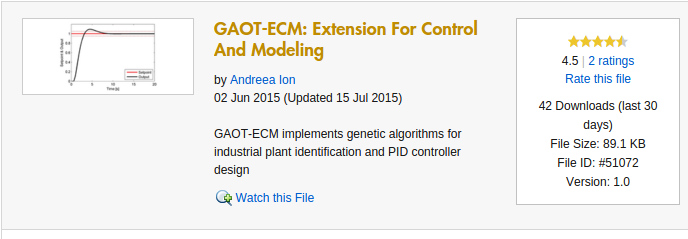
\includegraphics[width=1\linewidth]{GAOT.png}
		\end{figure}
		\end{frame}
		\begin{frame}
			\Huge{\centerline{The End}}
		\end{frame}
\end{spacing}
%------------------------------------------------
\end{document} 
